\documentclass[../main/main.tex]{subfiles}

\newdate{date}{18}{10}{2019}

\begin{document}

\chapter{Recall of statistical mechanics and theory of ensembles}
\marginpar{ \textbf{Lecture 4.} \\  \displaydate{date}. \\ Compiled:  \today.}

\section{Statistical ensembles}
Statistical mechanics roughly speaking was born as a sort of theory from microscopic trying to compute the macroscopic length using thermodynamics. The problem is going from the countinuous problems to the macroscopic problems. In origin was statistical mechanics of equilibrium system. Each microstate with a given energy fixed, will have the same probability, this is the equal probability statement.

\subsection{Microcanonical ensemble}
In general, if we consider a system with \emph{N,V} (number of particles and volume) fixed and also the total energy \emph{E} fixed, we call \( \Omega (E,V,N) \)  the number of microstate with total energy \emph{E} , volume \emph{V} and number of particles \emph{N}.

If the system is \emph{isolated} and in \emph{equilibrium} the rule of \textbf{equal probability} of the microstates holds:
\begin{orangebox}
If the system is isolated and in equilibrium with energy \emph{E} it visits each microstate consistent with energy \emph{E} with equal probability.
\end{orangebox}
Another way to say is: the system spends the same amount of time in each of the \( \Omega (E,V,N) \) microstates.

Therefore, we call  a single configuration of a given microstate \( \mathcal{C}  \). A configuration is just when you have the spatial part, because momentum can be obtained by integrating.
Let us suppose to compute the probability of a given configuration \( \mathcal{C}  \), \( P_{\mathcal{C}} \); because of equal probability we have:
\begin{equation}
  P_{\mathcal{C}} = \frac{1}{\Omega (E,V,N)}
  \label{eq:}
\end{equation}


Now, let us now consider two subsystem 1 and 2 that can exchange energy, volume and/or particles.
The number of microstates, of the combined system, of total energy \( E_T = E_1 + E_2 \), total volume \( V_T = V_1 + V_2 \) and \( N_T = N_1 + N_2 \) is given by:
\begin{equation}
  \Omega (E_T,V_T,N_T) = \sum_{E_1,V_1,N_1}^{} \Omega _1 (E_1,V_1,N_1) \Omega _2 (E_T - E_1,V_T-V_1,N_T-N_1)
\end{equation}
One can show that, in the thermodynamic limit, \(  \Omega (E_T,V_T,N_T) \) is strongly peaked around a given point \( (E_1^*,V_1^*,N_1^*) \) and the fluctuations around this value are rare and small. Writing \( \Omega (E_T,V_T,N_T)  \) as
\begin{equation}
  \Omega (E_T,V_T,N_T) \propto e^{\frac{S(E_T,V_T,N_T) }{k_B}} = \sum_{E_1,V_1,N_1}^{} \exp[ \frac{1}{k_B} (S_1 (E_1,V_1, N_1) + S_2 (E_2,V_2, N_2) ) ]
\end{equation}
(the proportionality becomes from the Boltzmann definition of entropy).

The values \( (E_1^*,V_1^*,N_1^*) \) are obtained by the max entropy condition that can be written as
\begin{subequations}
\begin{align}
  \dv{\ln{\Omega _1} }{E_1}  &= \dv{\ln{\Omega _2} }{E_2} \Rightarrow  T_1 = T_2 \\
  \dv{\ln{\Omega _1} }{V_1}  &= \dv{\ln{\Omega _2} }{V_2} \Rightarrow  P_1 = P_2 \\
  \dv{\ln{\Omega _1} }{N_1}  &= \dv{\ln{\Omega _2} }{N_2} \Rightarrow  \mu _1 = \mu _2
\end{align}
\end{subequations}
We next consider these properties to the case in which 1 is the system we want to study and 2 is a much larger system than 1 (a bath). This setup will bring us to the \emph{canonical ensemble}.

\section{The canonical ensemble}

\begin{figure}[h!]
\centering
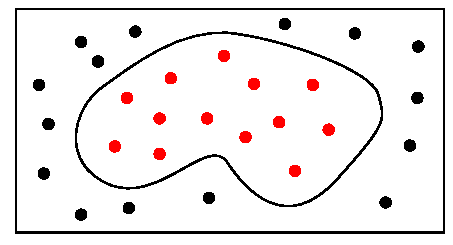
\includegraphics[width=0.6\textwidth]{../lessons/4_image/1.pdf}
\caption{\label{fig:4_1} Isolated system. There are two subsystems, \( S \)  constituted by red points and \( B \) constituted by the black one.}
\end{figure}

Let us consider an isolated system made by two subsystems, one \emph{S} and one much larger, \emph{B}, that we call \emph{thermal bath} (Figure \ref{fig:4_1}). The total number of particles is given by \( N_T = N_B + N_S\)  with \( N_B \gg N_S \gg 1 \) (they are both large but \emph{B} is much larger than \emph{S}), where \( N_B \) are the particles in the thermal bath and \( N_S \) the particle of the system.

Let \( E_T \) be the energy of the composite system. The two subsystems can exchange energy but the whole system has constant energy  \( E_T \). Therefore, let the energy to be free to fluctuate in time at fixed temperature  \( T_B \) (isothermal ensembles).
Note that \( V_S,N_S,V_B,N_B \) are fixed (no exchange of volume and particles).

For resuming, other quantities fixed are the temperature of the bath \( T_B \) , the number of the total particles of the system \( N_T \), and also the total volume \( V_T \).
 We have also \( V_T = V_B + V_S \), with   \( V_B \gg V_S \).

The key to the canonical formalism is the determination of the probability distribution of the system among its microstates. And this problem is solved by the realization that the system plus the bath constitute a closed system, with fixed temperature, to which the principle of equal probability of microstates applies.

If one assumes that the system and the bath are \emph{weakly coupled} (neglet interaction energy):
\begin{equation*}
  E_T = E_S + E_B = const \qquad E_B \gg E_S
\end{equation*}

Let \( \mathcal{C}  \) by the microstate of the system \( S \), and \( \mathcal{G}  \) the microstate of the heat bath \( B \).
A given microstate of the isolated composite system \emph{B-S} is given from a pair \( (\mathcal{C},\mathcal{G}  ) \) of microstate \( \mathcal{C} \in S  \) and   \( \mathcal{G} \in B  \).
The number of microstates of the isolated system with total energy \( E_T \) and system energy \( E_S \)  is given by:
\begin{equation*}
  \Omega _T (E_T,E_S) = \Omega (E_S) \Omega _B (E_T - E_S)
\end{equation*}
\begin{remark}
In this analysis \emph{V} and \emph{N} are fixed. Since \( E_T \) is fixed
\begin{equation}
  \Omega _T (E_T) = \sum_{E_S}^{} \Omega (E_S) \Omega _B (E_T - E_S)
\end{equation}
\end{remark}
From the principle of equal probability for microstates at equilibrium, the probability of a composed microstate \( (\mathcal{C} \circ \mathcal{G}  ) \) is given by:
\begin{equation}
P_{\mathcal{C} \circ \mathcal{G}} =
  \begin{cases}
   \frac{1}{\Omega _T (E_T)} & E_{\mathcal{C} } + E_{\mathcal{G} } = E_T \\
  0 & \text{otherwise}
  \end{cases}
\end{equation}
Since we are not interested to the microstates of the heat bath
\begin{equation}
  P_{\mathcal{C} } = \sum_{\substack{ \text{all } \mathcal{G}  \\  \text{such that}  \\ g (E_T -E_{\mathcal{C} } - E_{\mathcal{G} }) } }^{} P_{\mathcal{C} \circ \mathcal{G}}   = 
  \sum_{\substack{ \text{all } \mathcal{G}  \\  \text{such that}  \\ g (E_T -E_{\mathcal{C} } - E_{\mathcal{G} }) } }^{} \frac{1}{\Omega _T (E_T)} = \frac{1}{\Omega _T} \sum_{\mathcal{G} }^{}   1
\end{equation}
The number of microstates \( \mathcal{G}  \) with energy \( E_{\mathcal{G} }= E_T - E_{\mathcal{C} } \) is given by:
\begin{equation*}
  \Omega _B (E_{\mathcal{G} }) = \Omega_B (E_T - E_{\mathcal{C} })
\end{equation*}
This implies that the probability of a given configuration is related to the number of microstate of the bath:
\begin{equation}
  \Rightarrow   P_{\mathcal{C} }= \frac{\Omega _B (E_T - E_{\mathcal{C} })}{\Omega _T (E_T)} \propto \Omega _B (E_T - E_{\mathcal{C} })
\end{equation}
It is more convenient to deal with the logarithmic of \( P_{\mathcal{C} } \) that is smoother
\begin{equation}
  \Rightarrow k_B \ln{\Omega _B (E_T - E_{\mathcal{C} })} = S_B
\end{equation}
This is the entropy of \emph{B} and is a function of \( N_B \). Since \( E_{\mathcal{C}} \ll E_B \simeq E_T \) we can expand \( S_B (E_T - E_{\mathcal{C} }) \) around \( x_0 = E_T \) by the small amount
\begin{equation*}
  \Delta \equiv x-x_0 = (E_B) - (E_T) = - E_{\mathcal{C} }
\end{equation*}
\begin{equation*}
  f(E_B) = f(E_T) +  \eval{\dv{f}{E_B}}_{E_B = E_T} (E_B-E_T) + \dots
\end{equation*}
Therefore:
\begin{equation}
  k_B \ln{\Omega _B (E_B) } = S_B (E_B) = S_B (E_T) - E_{\mathcal{C} } \qty(\pdv{S_B}{E_B} )_{E_B = E_T} + \frac{E^2_{\mathcal{C} }}{2} \qty( \pdv[2]{S_B}{E_B} )_{E_B =E_T} + \dots
\end{equation}
To make explicit the \( N_B \) dependence, let us consider the molar version
\begin{equation*}
  S_B \rightarrow N_B s_B \qquad
  E_B \rightarrow N_B e_B
\end{equation*}
\begin{equation*}
  S_B =  N_B s_B = N_B s_B (E_T) - E_{\mathcal{C}} \qty(\pdv{s_B}{e_B} )_{e_B=e_T} + \frac{E_{\mathcal{C}}^2}{2 N_B}  \qty(\pdv[2]{s_B}{e_B} )
\end{equation*}
Let us consider the limit in which the system size is fixed, while the one of the heat bath is going to \( \infty  \):
\begin{subequations}
\begin{align}
  \lim_{N_B \rightarrow \infty } & \frac{E_T}{N_B} = \frac{E_S+ 
  \overbrace{N_B e_B}^{E_B}}{N_B} \rightarrow e_B \\
  \lim_{N_B \rightarrow \infty } & k_B \ln{\Omega _B (E_T - E_{\mathcal{C}})} \rightarrow N_B s_B - E_{\mathcal{C}} \dv{s_B}{e_B}
\end{align}
\end{subequations}
On the other hand,
\begin{equation*}
  \dv{s_B}{e_B} \equiv \frac{1}{T_B} = \frac{1}{T}
\end{equation*}
which implies
\begin{equation*}
  P_{\mathcal{C}} \propto \Omega _B (E_T - E_{\mathcal{C}}) 
  = \exp (\frac{S_B}{k_B})
  = \exp (\frac{N_B s_B}{k_B}- \frac{E_{\mathcal{C}}}{k_B T})
\end{equation*}
Since the first therm does not depend on \( \mathcal{C} \), it can be absorbed in the constant and what we get by expanding considering the huge number of particles
\begin{equation}
  P_{\mathcal{C}} \propto \exp (-E_{\mathcal{C}}/k_B T)
  \label{eq:4_1}
\end{equation}
\begin{remark}
Since the energy of the system fluctuates, its microstates are not anywhere equiprobable, but are visited with probability given by \eqref{eq:4_1}.
\end{remark}
\begin{remark}
Since the bath is very large, \emph{T} is the only property of the bath that affects the system. The \textit{Boltzmann factor} is defined as:
\begin{equation}
  \beta \equiv \frac{1}{k_B T}
\end{equation}
\end{remark}
The normalization consists in dividing by the normalization factor, that is the sum of all microstates
\begin{equation}
  P_{\mathcal{C}} = \frac{e^{-\beta E_ \mathcal{C}}}{\sum_{\mathcal{C}}^{} e^{-\beta E_ \mathcal{C}} }
  \label{eq:4_4}
\end{equation}
Finally, the \textbf{canconical partition function} is defined as
\begin{empheq}[box=\myyellowbox]{equation}
  Q(T,V,N) \equiv \sum_{\substack{ \text{all } \mathcal{C} \\  \text{with } V,N \\ \text{fixed}} }^{}  \exp (-\beta E_{\mathcal{C}})
  \label{eq:4_2}
\end{empheq}
Given \( Q(T,V,N) \), one gets the equation that states the link between statistical mechanics and thermodynamics, which is the \emph{Helhmoltz free energy}:
\begin{empheq}[box=\myyellowbox]{equation}
  A(T,V,N) = - k_B T \ln{Q(T,V,N)}
  \label{eq:4_3}
\end{empheq}
that is the free energy describing the isothermal (or canonical) ensemble at fixed \emph{T}, volume \emph{V} and number of particles \emph{N}.
\begin{remark}
\begin{equation*}
  Q(T,V,N) = \sum_{\substack{ \mathcal{C} \\ V,N \text{fixed} }} e^{-\beta E (\mathcal{C})} = \sum_{E}^{} e^{-\beta E} \Omega (E,V,N)
\end{equation*}
What we have done is a \emph{foliation} in energy of the space, that is a sum over the energy (keeping \( \{V,N\} \) fixed):
\begin{equation*}
  Q(T,V,N) = \sum_{E}^{} e^{-\beta E} \Omega (E,V,N) = \sum_{E}^{} e^{-\beta E} e^{S/k_B} = \sum_{E}^{} e^{-\beta (E-T S)}
\end{equation*}
Hence,
\begin{equation*}
  Q(T,V,N) = e^{-\beta A} \quad \Rightarrow A = - k_B T \ln{Q(T,V,N)}
\end{equation*}
\end{remark}

We have formulated a complete algorithm for the calculation of a fundamental relation in the canonical formalism. Given a list of states of the system, and their energies \( E_ {\mathcal{C}} \), we calculate the partition function \eqref{eq:4_2}. The partition function is thus obtained as a function of temperature and of the parameters that determine the energy levels. The fundamental relation is \eqref{eq:4_3} that determines the Helmholtz potential.

The probability of a configuration can be written as \eqref{eq:4_4}, that is a very useful form. Indeed, the average energy is expected to be
\begin{equation}
  U = \sum_{\mathcal{C}}^{} E_ {\mathcal{C}} P_{\mathcal{C}}  = \frac{ \sum_{\mathcal{C}}^{} E_ {\mathcal{C}} e^{-\beta E_ \mathcal{C}}}{\sum_{\mathcal{C}}^{} e^{-\beta E_ \mathcal{C}} }
\end{equation}
or
\begin{equation}
  U =  -\pdv{}{\beta } \ln{Q}
\end{equation}

\subsection{Energy fluctuations in the canonical ensemble}
Despite energy in the canonical ensemble fluctuates, while in the microcanonical one is constant, this does not contradict the equivalence principle of the ensemble (in the thermodynamic limit). The reason is that the relative size of the energy fluctuation decreases in the large system limit. 
To see it, let us compute the average square fluctuations of \emph{E}.
\begin{equation}
\expval{(\delta E)^2} = \expval{(E- \expval{E} )^2} = \expval{E^2} - \expval{E}^2
\end{equation}
\begin{remark}
Remember that thermodynamic assume that the number of number of freedom is related to the number of Avogadro.
\end{remark}
On the other hand,
\begin{equation*}
  \expval{E} = \sum_{\mathcal{C}}^{} P_{\mathcal{C}} E_{\mathcal{C}} = \sum_{\mathcal{C}}^{} E_{\mathcal{C}} \frac{e^{-\beta E_{\mathcal{C}}} }{\sum_{\mathcal{C}}^{} e^{-\beta E_{\mathcal{C}}}  }
   = - \qty( \frac{\pdv{Q (T,V,N)}{\beta }}{Q} ) = - \qty(\pdv{}{\beta } \ln{Q})_{N,V}
\end{equation*}
\begin{equation*}
  \expval{E^2} = \sum_{\mathcal{C}}^{} P_{\mathcal{C}} E_{\mathcal{C}}^2 = \frac{\qty(\pdv[2]{Q}{\beta } )}{Q}
\end{equation*}
Therefore,
\begin{equation*}
\begin{split}
  \expval{(\delta E)^2} = \expval{(E- \expval{E} )^2}  &= \frac{1}{Q} \qty(\pdv[2]{Q}{\beta } )_{N,V} - \frac{1}{Q^2} \qty(\pdv{Q}{\beta } )^2_{N,V}\\
  & =  \qty( \pdv[2]{\ln{Q} }{\beta} )_{N,V} = - \qty(\pdv{\expval{E} }{\beta } )_{N,V}
\end{split}
\end{equation*}
Since
\begin{equation}
  c_V = \qty(\pdv{E}{T} )_{N,V}
\end{equation}
we have
\begin{equation}
  \expval{(\delta E)^2} = k_B T^2 c_V
\end{equation}
Both \( c_V \) and \( \expval{E}  \) are extensive
\begin{equation*}
  \frac{\sqrt{\expval{(\delta E)^2} } }{\expval{E} } = \frac{\sqrt{k_B T^2 c_V} }{\expval{E} } \sim O \qty(\frac{1}{\sqrt{N} }) \Rightarrow 0
\end{equation*}
because \( N \sim 10^{23} \).



\section{Isothermal and isobaric ensemble}
Now, the system is coupled both to a thermal and a volumic bath at temperature \( T_B \) and pressure \( P_B \).
The idea is: consider the same system with the bath; the difference is that in this case the system can exchange energy but also volume (we continue to keep the temperature of the bath fixed). At this point the ensemble is \emph{isothermal} and \emph{isobaric}. All the assumptions done before are valid, in particular, assuming as before \emph{weak coupling} between the degrees of freedom of the bath and those of the system
\begin{subequations}
\begin{align*}
  E_T &= E + E_B \\
  V_T &= V + V_B
\end{align*}
\end{subequations}
We look for the partition function that describes this isothermal and isobaric ensemble.
Similarly to the previous case, one can write
\begin{equation}
  P_{\mathcal{C}} \propto  \Omega _B (E_B,V_B) \propto \Omega _B (E_T-E_{\mathcal{C}}, V_T - V_{\mathcal{C}}) \propto \exp [S_B (E_T - E_{\mathcal{C}},V_T - V_{\mathcal{C}})/k_B]
\end{equation}

\begin{remark}
Now, \( \mathcal{C} \) is specified both by its volume \emph{V} and energy \emph{E}. As before, one can expand \( \log \Omega _B   \)   both in \( E_B \) and in \( V_B \) (around \( E_T \) and \( V_T \)) and take the limit \( N_B \rightarrow \infty  \).
\end{remark}
\begin{equation}
  P_{\mathcal{C}} \propto \exp[ \frac{S_B (E_T,V_T)}{k_B}- \frac{E_{\mathcal{C}}}{k_B} \eval{\pdv{S_B}{E_B}}_{E_T,V_T} - \frac{V_{\mathcal{C}}}{k_B} \eval{\pdv{S_B}{V_B}}_{V_T,E_T} + \qty(term \simeq \frac{1}{N_B})]
\end{equation}
Recalling that
\begin{equation}
  \eval{\dv{S}{V} }_E = \frac{P}{T} \qquad \text{with } \begin{cases}
    P_B \rightarrow P \\ T_B \rightarrow T
\end{cases}
\end{equation}
\begin{equation}
  \Rightarrow P_{\mathcal{C}} \propto \exp [-\frac{E_{\mathcal{C}}}{k_B T} - \frac{P V_{\mathcal{C}}}{k_B T}]
\end{equation}
If we normalize:
\begin{equation}
  P_{\mathcal{C}} = \frac{e^{-\beta (E_{\mathcal{C}}+P V_{\mathcal{C}})}}{\Delta (T,P,N)}
\end{equation}
where
\begin{empheq}[box=\myyellowbox]{equation}
\Delta (T,P,N) = \sum_{\mathcal{C}}^{} e^{-\beta (E (\mathcal{C})+P V (\mathcal{C}))}
\end{empheq}
is called the \textbf{Gibbs partition function}.

\begin{remark}

Note that
\begin{equation*}
\begin{split}
\Delta (T,P,N)  &=  \sum_{V}^{} e^{-\beta PV } (\sum_{\substack{ \mathcal{C} \\ V,N \text{fixed}} }^{} e^{-\beta E_{\mathcal{C}}}  ) =  \sum_{V}^{} e^{-\beta PV} Q (T,V,N)       \\
& = \underbrace{\sum_{V}^{} \sum_{E}^{}}_{\substack{ \text{fluctuating} \\  \text{variables} } }  e^{-\beta (E+PV)} \Omega (E,V,N)
\end{split}
\end{equation*}
By summing over all the microstates compatible with \emph{E} and \emph{V}:
\begin{equation}
  P (E,V) = \frac{\Omega (E,V,N)}{\Delta (T,P,N)} e^{-\beta (E+PV)}
\end{equation}
\end{remark}
\begin{remark}
\begin{equation}
  \Delta (T,P,N) = \underbrace{ \sum_{E}^{} \sum_{V}^{} e^{-\beta E - \beta PV}}_{\text{Laplace transform}} \Omega (E,V,N) = \sum_{E,V}^{} e^{-\beta E- \beta PV + S(E,V,N)/k_B}
  \label{eq:4_5}
\end{equation}
\end{remark}




\subsubsection{Classical systems (fluids)}
\begin{equation}
  \Delta (T,P,N) = \int_{0}^{\infty } \dd[]{V} e^{-\beta PV} \qty[ \frac{1}{h^{3N}N!} \int_{}^{} \dd[]{\va{p_1}} \dots \dd[]{\va{p_N}} e^{-\beta \mathcal{H}(p^N,r^N)} ]
\end{equation}
which implies
\begin{equation}
  \Delta (T,P,N) = \int_{0}^{\infty } \dd[]{V} e^{-\beta PV} Q(T,V,N)
\end{equation}
that is the Laplace transform of the canonical partition function \emph{Q}.  

We also define
\begin{equation}
  \beta P \equiv \frac{P}{T} = \pdv{S}{V}
\end{equation}
\begin{remark}
Let us remind that
\begin{definition}{Laplace transform}{}
The Laplace transform of a function \(f(t) \), defined for all real numbers \(t \geq 0\), is the function \(F(s)\), which is a unilateral transform defined by
\begin{equation*}
 F(s)=\int _{0}^{\infty }f(t)e^{-st}  \dd[]{t}	
 \end{equation*}
 where \(s\) is a complex number frequency parameter  with real numbers \( \sigma \) and \( \omega \):
\begin{equation*}
    s=\sigma +i\omega 
\end{equation*}
\end{definition}
\end{remark}

\subsubsection{Magnetic system}
Ensemble in which both \emph{E} and \emph{M} can fluctuate. In particular, we have \( \Omega (E,M) \) (with \( T_B \) and \( H_B \) fixed).
\begin{equation}
  P_{\mathcal{C}} \propto e^{ \frac{S_B (E_T,M_T)}{k_B} - \frac{E_{\mathcal{C}}}{k_B}\dv{S_B}{E_B} - \frac{M_{\mathcal{C}}}{k_B} \dv{S_B}{M_B}  }
\end{equation}
Since \( \dv{S_B}{M_B} = -\frac{H_B}{T_B}   \) and \( \dv{S_B}{E_B} = \frac{1}{T_B}  \):
\begin{equation}
  \Rightarrow P_{\mathcal{C}} \propto \exp [-\beta (E_{\mathcal{C}}-H M_{\mathcal{C}})], \qquad T_B \rightarrow T, H_B \rightarrow H
\end{equation}
The normalization function is:
\begin{equation}
  \Delta (T,H,N) = \sum_{\mathcal{C}}^{} e^{-\beta (E_{\mathcal{C}}-H M_{\mathcal{C}})} = \sum_{E,M}^{} e^{-\beta E + \beta M H} \Omega (E,M)
  \label{eq:4_6}
\end{equation}
that is the \emph{Gibbs partition function} for magnetic systems.



\subsection{Saddle point approximation}
The sum \eqref{eq:4_5} can be approximated by the maximum of the integrand (this is fair for highly peaked functions):
\begin{equation*}
  \sum_{E,V}^{} \exp [-\beta E- \beta PV + S(E,V,N)/k_B] \approx e^{-\beta E^* - \beta PV^* + S(E^*,V^*,N)/k_B}
\end{equation*}
where
\begin{equation*}
  \qty(\dv{S(E^*,V^*,N)}{E} )_{V,N} = \frac{1}{T}, \qquad \qty(\dv{S(E^*,V^*,N)}{V} )_{E,N} = \frac{P}{T}
\end{equation*}
this implies
\begin{equation*}
  -k_B T \ln{\Delta (T,P,N)} \simeq E^* + PV^* - TS
\end{equation*}
Hence, we define the \textbf{Gibbs free energy} as:
\begin{empheq}[box=\myyellowbox]{equation}
  G(T,P,N) = - k_B T \ln{\Delta (T,P,N)}
\end{empheq}


\section{Gran canonical ensemble}
In this case \emph{N} varies instead than \emph{V}. Thus we have
\begin{equation}
\begin{split}
P_{\mathcal{C}}  &= \exp [\frac{S_B (E_T - E_{\mathcal{C}},N_T - N_{\mathcal{C}})}{k_B}] \\
& \sim \exp [\frac{S_B(E_T,N_T)}{k_B}- \frac{E_{\mathcal{C}}}{k_B} \dv{S_B}{E_B}- \frac{N_{\mathcal{C}}}{k_B} \dv{S_B}{N_B} + \qty(\text{terms of order} \le \frac{1}{V_B}) ] \\
& = \frac{\exp [-\beta E_{\mathcal{C}}+ \beta \mu N_{\mathcal{C}}] }{\Theta (T,V,\mu )}
\end{split}
\end{equation}
where
\begin{empheq}[box=\myyellowbox]{equation}
  \Theta (T,V,\mu ) = \sum_{N}^{} \sum_{\substack{\mathcal{C} \\ V,N \text{fixed}} }^{} e^{-\beta (E_{\mathcal{C}}- \mu N)}
\end{empheq}
is the \textbf{grancanonical partition function}.
\begin{remark}
Remember that
\begin{equation}
  \dv{S}{E} = \frac{1}{T}, \qquad \dv{S}{N} = \frac{\mu }{T}
\end{equation}
\end{remark}
The \emph{fugacity} is defined as:
\begin{equation}
  z \equiv e^{\beta \mu }
\end{equation}
and we rewrite
\begin{equation}
    \Theta (T,V,\mu ) = \sum_{N=0}^{\infty } z^N (\sum_{\substack{\mathcal{C} \\ V,N \text{fixed}} }^{} e^{-\beta E_{\mathcal{C}}}  )
\end{equation}

In principle, if one is able to compute the partition function is able to compute the thermodynamic quantitites.


\end{document}
